\documentclass[PhD-Yoann-Dupont.tex]{subfiles}
\begin{document}

La seconde approche utilisée dans le TAL est l'apprentissage automatique, que nous pouvons définir comme l'ensemble des méthodes faisant qu'une machine va s'améliorer par l'expérience \citep{cornuejols2011apprentissage}. Plus précisément, nous nous concentrerons sur l'apprentissage automatique dit supervisé, où des exemples de la tâche à accomplir sont donnés en entrée à un algorithme qui inférera alors des règles basées sur des statistiques afin de pouvoir adhérer au mieux aux exemples qui lui ont été donnés.

D'un point de vue formel, nous disposons de données X issues d'une distribution P$_{X}$, un oracle qui utilise la fonction $f$ à apprendre pour étiqueter les données de X et d’une fonction $h$ qui est la fonction apprise à partir de ces exemples. L’espace des observations S de taille m est défini comme <(x$_{i}$, f(x$_{i}$))>$_{1\leq i \leq m}$. il existe deux grands cas dans lesquels on emploie cette forme d’apprentissage comme :
\begin{itemize}
    \item problème de régression : il s’agit de trouver une fonction $h$ qui se rapproche de $f$. Autrement dit : $\forall\ x \in X, h(x) \approx f(x) = y$
    \item apprentissage d’une classification : l’espace de sortie de $f$ est un ensemble discret dont la cardinalité est le nombre de classes/étiquettes à apprendre. Un cas particulier de classification est l'\emph{annotation de séquences}, qui sera l'intérêt de la thèse.
    %\item apprentissage de concepts : nous cherchons à reconnaître une classe précise, l’image de $f$ étant les booléens pour décrire l’objet comme faisant ou non partie de la classe à apprendre.
    %\item problème d’optimisation multi-critères : quand plusieurs objectifs sont à maximiser.
\end{itemize}

L'illustration du processus général d'apprentissage automatique est décrit dans la figure\ \ref{fig:machine-learning-general}.

\begin{figure}[ht!]
\centering{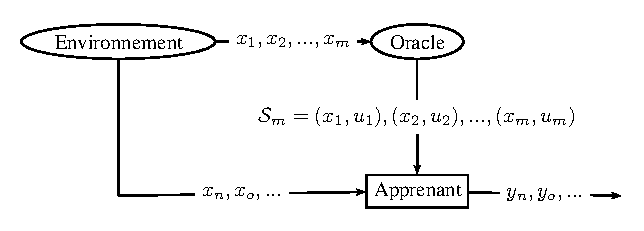
\includegraphics[scale=1.0]{images/rules-vs-learning/apprentissage-automatique}}
\begin{itemize}
    \item x$_{1}$, x$_{2}$, ..., x$_{m}$, x$_{n}$, ... : les données non étiquetées. %Par exemple, x$_{i}$ = «\ Yoann Dupont fait une thèse à Paris 3 .\ »
    \item l’oracle associe des étiquetages y$_{i}$ = f(x$_{i}$) à chaque x$_{i}$, fournissant une observation de référence S$_{m}$. des exemples sont donnés dans les figure \ref{tab:POS-tagging-example}, \ref{tab:NP-chunking-example} et \ref{tab:ner-example}.
    \item à partir de ces données de référence, l’apprenant cherche à inférer la fonction f, le résultat de cet apprentissage donnant la fonction h. Ici, h représente une fonction d’étiquetage apprise à partir des données. Une fois apprise, l’apprenant utilise la fonction h pour calculer des séquences d’étiquettes y$_{i}$ = h(x$_{i}$) corespondant à chaque x$_{i}$.
\end{itemize}
\caption{description général du processus d'apprentissage}
\label{fig:machine-learning-general}
\end{figure}

Dans ce cadre, la REN est typiquement formulée comme une tâche d'annotation de séquences, où nous disposons d'un ensemble de tokens organisés selon une structure connue ou sous-jacente, auxquels nous souhaitons associer une étiquette afin de les caractériser. Afin d'illustrer ce à quoi ressemble une tâche d'annotation, prenons d'abord le cas plus simple qu'est l'annotation morphosyntaxique, où le but est de trouver la nature de chaque token dans une phrase. Reprenons l'exemple précédent «\ Yoann Dupont fait une thèse à Paris 3.\ », qui se verra alors formulé en tâche d'annotation morphosyntaxique de la façon suivante :

\begin{table}[ht!]
\centering
\begin{tabular}{lccccccccc}
x$_{i}$ & Yoann & Dupont & fait & une & thèse & à & Paris & 3 & . \\
        & $\downarrow$ & $\downarrow$ & $\downarrow$ & $\downarrow$ & $\downarrow$ & $\downarrow$ & $\downarrow$ & $\downarrow$ & $\downarrow$ \\
y$_{i}$ & nom-p & nom-p & verbe & dét & nom-c & prép & nom-p & adj & ponct \\
\end{tabular}
\caption{exemple d'étiquetage morphosyntaxique}
\label{tab:POS-tagging-example}
\end{table}

Nous remarquons que chaque token a sa propre étiquette, cette représentation semble donc plutôt inadaptée pour une tâche de REN de prime abord, «\ Paris 3\ » étant une entité s'étendant sur plusieurs tokens. Il est cependant possible de simuler l'annotation des données par groupes, ces groupes étant alors des sous-chaînes de la séquence globale. Pour ce faire, différent marqueurs sont concaténés à l'étiquette : B (Begin) marquant le début d'un groupe nominal, I (In) marquant l'appartenance à un groupe précédemment commencé et O (Out) marque tout ce qui n'appartient à aucun groupe. Il n'y a pas de marqueur de fin explicite car la fin d'un groupe se déduit soit par le début d'un autre groupe soit par une arrivée sur un non-groupe. Ce schéma d'annotation est régulièrement utilisé car il s'agit du plus simple capable de représenter de façon exacte les groupes. Dans l'exemple suivant, nous effectuons un étiquetage des groupes nomninaux :

\begin{table}[ht!]
\centering
\begin{tabular}{lccccccccc}
x$_{i}$ & Yoann & Dupont & fait & une & thèse & à & Paris & 3 & . \\
        & $\downarrow$ & $\downarrow$ & $\downarrow$ & $\downarrow$ & $\downarrow$ & $\downarrow$ & $\downarrow$ & $\downarrow$ & $\downarrow$ \\
y$_{i}$ & B & I & O & B & I & O & B & I & O \\
\end{tabular}
\caption{exemple d'étiquetage en chunks nominaux}
\label{tab:NP-chunking-example}
\end{table}

En associant ces marqueurs de position avec un identifiant, il est alors possible de modélider la reconnaissance d'entités nommées en tant que tâche d'annotation, la phrase pouvant alors être annotée de la façon suivante :

\begin{table}[ht!]
\centering
\begin{tabular}{lccccccccc}
x$_{i}$ & Yoann & Dupont & fait & une & thèse & à & Paris & 3 & . \\
        & $\downarrow$ & $\downarrow$ & $\downarrow$ & $\downarrow$ & $\downarrow$ & $\downarrow$ & $\downarrow$ & $\downarrow$ & $\downarrow$ \\
y$_{i}$ & B-Personne & I-Personne & O & O & O & O & B-Organisation & I-Organisation & O \\
\end{tabular}
\caption{exemple d'étiquetage en entité nommées}
\label{tab:ner-example}
\end{table}

Supposons que la fonction apprise ne soit pas parfaite et ne reconnaisse pas «\ Paris 3\ » comme une organisation, mais reconnaisse à la place «\ Paris\ » comme un lieu. Nous aurions :

\begin{table}[ht!]
\centering
\begin{tabular}{lccccccccc}
x$_{i}$ & Yoann & Dupont & fait & une & thèse & à & Paris & 3 & . \\
        & $\downarrow$ & $\downarrow$ & $\downarrow$ & $\downarrow$ & $\downarrow$ & $\downarrow$ & $\downarrow$ & $\downarrow$ & $\downarrow$ \\
h$_{i}$ & B-Personne & I-Personne & O & O & O & O & B-Lieu & O & O \\
\end{tabular}
\caption{exemple d'étiquetage en entité nommées}
\label{tab:ner-tagging-example}
\end{table}

Ces erreurs faites par l'algorithme d'apprentissage sont la base du processus d'apprentissage : lorsqu'il commet une erreur, l'algorithme s'ajuste afin de la corriger. Ainsi, avec suffisamment d'exemples, nous supposons que l'algorithme sera en mesure de généraliser l'information qu'il a obtenue dans son espace des observations $S$, et de ne pas se contenter de reproduire les exemples qu'il a à sa disposition. Dans la section suivante, nous présenterons les différents algorithmes d'apprentissage automatique que nous avons étudiés dans le cadre de cette thèse.

\end{document}